\subsection{Prototyper med fokus på systemets funktionalitet}
\label{subsec:prototype2}
\tjek{Revideret af Elias d. 11.12.12}

Systemet kan ikke blot fungere med en søgefunktion. Der skal flere funktioner til før systemet er brugbart. Til at test disse andre funktioner, brugte vi en diasshow-prototype, som er dynamisk, hvilket giver en fornemmelse af et fungerende system. Denne prototype kalder vi for prototype 2, og den er vist på \figref{fig:prototype2design}. Testene af prototyperne i \secref{subsec:prototype1} havde til formål at give os mulighed for at træffe et kvalificeret valg i forhold til, hvilken søgefunktion, vi skulle benytte os af på forsiden af systemet. Derfor er der i dette afsnit fokus på den side, hvor resultaterne af en søgning skal vises.

Figur \ref{fig:prototype2design} viser opskrifter, der er resultatet af en søgning, som er blevet udført af informanten. Opskrifterne er blot eksempler, som vi selv har lavet for at få fyldt lidt tekst på siden. Der var fokus på, hvorvidt informanterne var i stand til at navigere rundt på siden, og undersøge om funktionernes placering, synlighed og brug var intuitiv for informanten.

\begin{figure}[H]
	\centering
	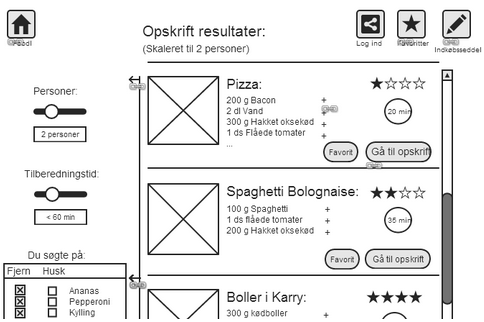
\includegraphics[scale=0.7]{billeder/prototyper/prototype2.png}
	\capt{Visualisering af prototype 2, der har fokus på systemets funktionalitet. Udviklet vha. \url{http://www.gomockingbird.com}.}
	\label{fig:prototype2design}
\end{figure}

I toppen af prototypen i \figref{fig:prototype2design} ses fire knapper. Fra venstre skal disse forestille en ``hjem''-knap, ``log ud/ind''-knap, ``favorit''-knap og en ``indkøbsliste''-knap. Vi har benyttet os af både figurer, der minder om den hændelse, der vil ske, når man klikker på knappen. Her benytter vi os af mennesker gode evne til at genkende objekter og deres bedtydning.\cite[p. ~340]{deb} Derudover er der også en kort beskrivelse af, hvad der sker, hvis man klikker. Begge informanter kunne forstå, hvad knapper i toppen af siden skulle bruges til. Merete var dog en smule i tvivl om ``favorit''-knappen havde til formål at tiltøje opskrifter til en favoritliste eller om den viste de favoritter, man havde gemt.

I venstre side af \figref{fig:prototype2design} ses en sidebar, hvor der er nogle funktioner til at manipulere søgeresultatet. Denne sidebar er normalt gemt, og man skal klikke på en tast i venstre side af søgeresultatet for at åbne sidebaren. Fra sidebaren er det bl.a. muligt at skalere opskrifter mht. antal personer, begrænse søgeresultatet i forhold til tilberedningstid eller i forhold til råvarer (dette er nyttigt, hvis man \fx er allergiker eller ikke spiser noget specifikt). Derudover kan man se sin nuværende søgning i sidebaren og fjerne eller huske de indtastede råvarer. Begge informanter havde problemer med at opdage, at der var en sidebar, fordi den var gemt væk. De var enige om, at den sagtens kunne forblive åben, når man havde udført en søgning. Informanterne var også enige om, at det ville være meget nyttigt med de forskellige funktioner til at manipulere opskrifterne med, men \fx ved skaleringsfunktionen behøvede man ikke at være i stand til at skalere til \fx 30 personer, da der netop var tale om brug af madrester. 

Som det ses på \figref{fig:prototype2design} så vises opskrifterne i en liste, og hver opskrift har nogle funktioner, der er tilknyttet til den ene opskrift. Herfra er det muligt at tilføje ingredienserne til en indkøbsliste vha. de små +'er ud for hver ingrediens. Derudover kan man favorisere en opskrift, så den er gemt i favoritlisten. Derudover kan man se, hvor populær en opskrift er ved de stjerner, der er ved hver opskrift, samt tilberedningstiden for den enkelte opskrift lige under. Når man har valgt en opskrift, så kan man gå til opskriftens hjemmeside, hvor fremgangsmåden kan findes. Merete havde ikke overvejet at +'et skulle bruges til at tilføje en ingrediens til indkøbslisten. Derudover var begge informanter enige om, at de nuværende funktioner var nyttige, og at det var helt fint, at man kun kunne se, hvilke ingredienser man skulle bruge og så navigere til den originale side for at se hele fremgangsmåden.

\subsection{Sammendrag}
Merete var en smule forvirret omkring brugen af knapperne i toppen af siden. Et forslag var, at vi kunne tilføje mere sigende tekst som ``Vis favoritter'' i stedet for, at der blot står ``Favoritter'' eller lignende. Informanterne synes også, at små funktioner som +'et, der bruges til at tilføje en ingrediens til indkøbslisten, skal være mere intuitiv.

Informanterne var enige om, at en så stor del af funktionalitet, som sidebaren er, skal være synlig igennem hele processen, fra man er på søgeresultatsiden. De mente ikke, at den skulle gemmes væk.

Derudover kunne informanterne godt finde ud af at bruge de andre funktioner på systemet.